\chapter{Где учатся и кем работают изобретатели языков программирования}
\label{ch:programming languages}

%\footnotetext{
\marginnote{Используемые в SPARQL-запросах объекты:
\begin{itemize}
	\item\href{https://www.wikidata.org/wiki/Q9143}{programming language}~--- язык программирования;
	\item\href{https://www.wikidata.org/wiki/Q899523}{object-based language}~--- объектно-ориентированный язык программирования.
\end{itemize}
Используемые в SPARQL-запросах свойства:
\begin{itemize}
	\item\href{https://www.wikidata.org/wiki/Property:P737}{influenced by}~--- какие языки программирования оказали влияние;
	\item\href{https://www.wikidata.org/wiki/Property:P178}{developer}~--- кто разработал язык программирования;
	\item\href{https://www.wikidata.org/wiki/Property:P275}{copyright license}~--- какая лицензия;
	\item\href{https://www.wikidata.org/wiki/Property:P31}{instance of}~--- к какому более общему типу (типам) относится этот язык;
	\item\href{https://www.wikidata.org/wiki/Property:P1195}{file extension}~--- расширение файлов;
	\item\href{https://www.wikidata.org/wiki/Property:P159}{headquarters location}~--- место расположения штаб-квартиры разработчиков языка;
	\item\href{https://www.wikidata.org/wiki/Property:P625}{coordinate location}~--- геокоординаты объекта;
	\item\href{https://www.wikidata.org/wiki/Property:P69}{educated at}~--- где учился объект;
	\item\href{https://www.wikidata.org/wiki/Property:P19}{place of birth}~--- где родился объект;
	\item\href{https://www.wikidata.org/wiki/Property:P106}{occupation}~--- род занятий объекта (профессия).
\end{itemize}
}

В работе исследуются свойства языков программирования на основе базы знаний международного проекта Викиданные. С помощью SPARQL-запросов, вычисляемых на объектах типа <<язык программирования>>  в Викиданных, решён ряд задач. Получены перечени всех языков программирования под пермиссивными лицензиями и языков с закрытыми лицензиями и рассчитано их процентное соотношение. Построена пузырьковая диаграмма по количеству разных расширений файлов для одного языка программирования. Получены карты, отображающие месторасположение учебных заведений и компаний, в которых учились или работали люди, связанные с созданием языков программирования. Построена пузырьковая диаграмма, отображающая популярные профессии среди людей, причастных к созданию и разработке языков программирования. Получен список всех объектно-ориентированных языков программирования и сделан вывод об исчерпывающей полноте Викиданных относительно них. Проведено сравнение и анализ результатов SPARQL-запросов 2017 года и 2020 года, отмечены основные изменения. 

%%
% Список языков программирования
%%
\section{Список языков программирования}
Выведем (листинг \ref{lst:prog_langs}) список всех языков программирования, с которыми будет вестись работа в дальнейшем. Для этого мы используем объект \wdqName{programming language}{9143} и свойство \href{https://www.wikidata.org/wiki/Property:P31}{instance of (P31)}.

\begin{lstlisting}[
	language=SPARQL,
	label=lst:prog_langs,
	caption={\href{https://w.wiki/uGs}{Список языков программирования}\protect\footnotemark},
	texcl 
]
#List of programming languages
SELECT ?lang ?langLabel
WHERE
{
    ?lang wdt:P31 wd:Q9143. # instances of programming language
    SERVICE wikibase:label { bd:serviceParam wikibase:language "ru"}
}
\end{lstlisting}
\footnotetext{Результатом запроса~\ref{lst:prog_langs} является список всех языков программирования. На 2017 год список содержал 732 записи, а на 2020 год число языков программирования увеличилось до \num{1422} записи. Ссылка на SPARQL-запрос: \href{https://w.wiki/uGs}{https://w.wiki/uGs}
}

На 2020 год наиболее проработанными на Викиданных языками программирования были: \href{https://www.wikidata.org/wiki/Q2407}{C++} (26 свойств), \href{https://www.wikidata.org/wiki/Q251}{Java} (26 свойств), \href{https://www.wikidata.org/wiki/Q2005}{JavaScript} (25 свойств), \href{https://www.wikidata.org/wiki/Q206904}{R} (25 свойств).
Почти пустыми и малоинформативными языками на 2020 год оказались\cite{prowd_langs_link}: \href{https://www.wikidata.org/wiki/Q3991643}{Tiny}, \href{https://www.wikidata.org/wiki/Q3924253}{Proteus}, \href{https://www.wikidata.org/wiki/Q21524853}{Comfy} --- всего по одному свойству.
Недостаток полученного списка в том, что ряд объектов получился безымянным на Викиданных (No label defined). Попробуем получить список языков, у которых поле label  будет непустым.

\label{question:prog_lang_1}
\marginnote{
Соотнесите язык программирования и его разработчика.
	\begin{tabular}{ll}
		Разработчик & Язык\\
		\hline
		\href{https://ru.wikipedia.org/wiki/Ишбиа,_Жан}{Жан Ишбиа} & \href{https://www.wikidata.org/wiki/Q154755}{Ада}\\
		\href{https://ru.wikipedia.org/wiki/Мур,_Чарльз_(программист)}{Чарльз Мур} & \href{https://www.wikidata.org/wiki/Q275472}{Форт}\\
		\href{https://ru.wikipedia.org/wiki/Армстронг,_Джо_(программист)}{Джо Армстронг} & \href{https://www.wikidata.org/wiki/Q334879}{Erlang}\\
	\end{tabular}
\newline
См. ответ~\ref{answer:prog_lang_1} на с.~\pageref{answer:prog_lang_1}.
}

\begin{lstlisting}[
	language=SPARQL,
	label=lst:labeled_languages,
	caption={\href{https://w.wiki/v2a}{Список языков программирования с заполненным свойством label}\protect\footnotemark},
	texcl
]
#List of programming languages with a label only
SELECT ?lang ?lang_label
WHERE
{
    ?lang wdt:P31 wd:Q9143
    ; rdfs:label ?lang_label FILTER (LANG(?lang_label) = "ru") . 
}
\end{lstlisting}
\footnotetext{Результатом запроса~\ref{lst:labeled_languages} также будет список языков программирования, но из него исключены те, для которых не указан параметр label на русском языке. На 2020 год в списке было 630 записей. Ссылка на SPARQL-запрос: \href{https://w.wiki/v2a}{https://w.wiki/v2a}}

%%
% Демонстрация работы с операциями над множества в SPARQL
%%
Теперь получим список (листинг~\ref{lst:free_license_languages}) всех языков программирования, являющихся открытым программным обеспечением (free software) и испытавших на себе влияние хотя бы одного из следующих языков программирования: \href{https://en.wikipedia.org/wiki/C_(programming_language)}{Си}, \href{https://ru.wikipedia.org/wiki/Python}{Python}, \href{https://ru.wikipedia.org/wiki/Java}{Java}. При этом в разработке этих языков не участвуют следующие две фирмы: \href{https://ru.wikipedia.org/wiki/Sun_Microsystems}{Sun Microsystems}, \href{https://en.wikipedia.org/wiki/Johnson_Space_Center}{Космический центр имени Линдона Джонсона}.

\index{SPARQL!MINUS!Список свободных языков программирования}
\begin{lstlisting}[
	language=SPARQL,
	label=lst:free_license_languages,
	caption={\href{https://w.wiki/v2n}{Список свободных языков программирования}\protect\footnotemark},
	texcl
]
SELECT DISTINCT ?prog ?progLabel
WHERE
{
  ?prog wdt:P31 wd:Q9143 # instance of programming language
  SERVICE wikibase:label { bd:serviceParam wikibase:language "ru" } 
  {
    { ?prog wdt:P737 wd:Q15777 } UNION # influenced by C
    { ?prog wdt:P737 wd:Q28865 } UNION # influenced by Python
    { ?prog wdt:P737 wd:Q251 } UNION # influenced by Java
    { ?prog wdt:P31 wd:Q341 }
  } MINUS
  { #developer
    { ?prog wdt:P178 wd:Q14647 } UNION # developer Sun Microsystems
    { ?prog wdt:P178 wd:Q208371 } # developer Lyndon Johnson Space Center
  }
}
\end{lstlisting}
\footnotetext{Рeзультатом запроса~\ref{lst:free_license_languages} является список языков программирования, удовлетворяющих указанным выше требованиям. На 2017 год список содержал 115 записей, на 2020 год~--- 125 записей. Ссылка на SPARQL-запрос: \href{https://w.wiki/v2n}{https://w.wiki/v2n}}

%%
% Пермиссивные лицензии
%%
Построим список языков программирования, находящихся под \href{https://en.wikipedia.org/wiki/Permissive_software_license}{пермиссивными лицензиями} (листинг~\ref{lst:permessive_license}).\marginnote{\index{Языки программирования!Определения!Пермиссивные лицензии} Пермиссивные лицензии на свободное программное обеспечение~--- это такие лицензии, которые почти не ограничивают свободу действий пользователей и разработчиков.}
\footnotetext{Результатом работы запроса~\ref{lst:permessive_license} является список языков программирования, находящихся под пермиссивными лицензиями. На 2017 год список содержал 37 записей, на 2020 год в списке 83 записи. В этот список из 83 <<свободных>>  языков попали, например \href{https://ru.wikipedia.org/wiki/CoffeeScript}{CoffeeScript}, \href{https://ru.wikipedia.org/wiki/Go}{Go}, \href{https://ru.wikipedia.org/wiki/Haml}{Haml}. Ссылка на SPARQL-запрос: \href{https://w.wiki/v3A}{https://w.wiki/v3A}}
\begin{lstlisting}[
	language=SPARQL,
	label=lst:permessive_license,
	caption={\href{https://w.wiki/v3A}{Языки программирования с пермиссивными лицензиями}\protect\footnotemark},
	texcl
]
SELECT DISTINCT ?lang ?langLabel
WHERE
{
    ?lang wdt:P31 wd:Q9143
    SERVICE wikibase:label { bd:serviceParam wikibase:language "ru" }.
    { ?lang wdt:P275 wd:Q308915  }  UNION  # license Mozzila Public
    { ?lang wdt:P275 wd:Q334661  }  UNION  # license MIT
    { ?lang wdt:P275 wd:Q191307  }  UNION  # license BSD
    { ?lang wdt:P275 wd:Q6905323 }         # license CC
}
\end{lstlisting}
Рассмотрим соотношение языков с пермиссивной лицензией и языков с проприетарными или закрытыми лицензиями.

\footnotetext{Рeзультатом запроса~\ref{lst:license_compare} будет значение отношения числа языков программирования со свободной лицензией к числу языков с закрытой лицензией. На 2020 год это значение равно 26\%. Ссылка на SPARQL-запрос: \href{https://w.wiki/v3B}{https://w.wiki/v3B}}
\label{question:prog_lang_2}
\marginnote[50pt]{
Приведённые ниже изображения~--- логотипы разных языков программирования. Какое из изображений является логотипом языка \href{https://www.wikidata.org/wiki/Q513238}{LOLCODE}?\newline
	\begin{tabular}{c}
		
\includegraphics[width=2cm]{./chapter/programming_language/task_2_logo_1.PNG}\\
		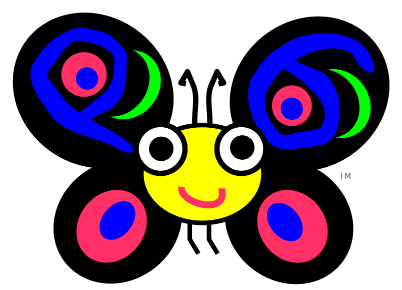
\includegraphics[width=2cm]{./chapter/programming_language/task_2_logo_2.PNG}\\
		
\includegraphics[width=2cm]{./chapter/programming_language/task_2_logo_3.PNG}\\
		
\includegraphics[width=2cm]{./chapter/programming_language/task_2_logo_4.PNG}\\
	\end{tabular}
\newline
См. ответ~\ref{answer:prog_lang_2} на с.~\pageref{answer:prog_lang_2}.
}
\begin{lstlisting}[
	language=SPARQL,
	label=lst:license_compare,
	caption={\href{https://w.wiki/v3B}{Расчёт отношения свободных языков к закрытым}\protect\footnotemark},
	texcl
]
#The script calculates the percentage of programming languages 
#with a free license in relation to languages with a closed license
SELECT (COUNT(?not_free)* 100 / (COUNT(?free)) as ?total) WHERE
{{
    SELECT ?free WHERE {
      ?free wdt:P31 wd:Q9143 # instances of programming language
       SERVICE wikibase:label { bd:serviceParam wikibase:language "ru" }
       { ?free wdt:P275 wd:Q308915  }  UNION  # license Mozilla Public
       { ?free wdt:P275 wd:Q334661  }  UNION  # license MIT
       { ?free wdt:P275 wd:Q191307  }  UNION  # license BSD
       { ?free wdt:P275 wd:Q6905323 }         # license CC
    }
} UNION {
    SELECT ?not_free WHERE {
      ?not_free wdt:P31 wd:Q9143 # instances of programming language
      SERVICE wikibase:label { bd:serviceParam wikibase:language "ru" }
      { ?not_free wdt:P275 wd:Q6165015 } UNION # Java Research License
      { ?not_free wdt:P275 wd:Q218616 } UNION # proprietary software
      { ?not_free wdt:P275 wd:Q3238057 } UNION # proprietary license 
      { ?not_free wdt:P275 wd:Q31202214 } UNION # proprietary software 
      { ?not_free wdt:P275 wd:Q979794 } # Aladdin Free Public License
    }}
}
\end{lstlisting}

Приведённый выше запрос состоит из двух подзапросов. Первый получает список свободных языков программирования, а второй~--- закрытых, после чего находится отношение числа языков в полученных списках.
%%
% Количество форматов файлов исходного кода
%%
\section{Количество форматов файлов исходного кода}
\marginnote{\index{Языки программирования!Определения!Расширение имени файла}Расширение имени файла~---~это последовательность символов, добавляемых к имени файла и предназначенных для идентификации типа (формата) файла. Это один из распространённых способов, с помощью которых пользователь или программное обеспечение компьютера может определить тип данных, хранящихся в файле, например: имя.jpg~---~это фотографии, имя.avi~---~видеофайл.}
В зависимости от языка программирования, файлы с исходным кодом программ могут иметь разные расширения. Построим~\ref{lst:source_formats} пузырьковую диаграмму по количеству допустимых форматов файлов исходного кода и сравним с аналогичной диаграммой, построенной в 2017 году.

\index{График!BubbleChart!Количество форматов файлов исходного кода}
\begin{lstlisting}[
	language=SPARQL,
	label=lst:source_formats,
	caption={\href{https://w.wiki/uGQ}{Количество форматов файлов исходного кода.}\protect\footnotemark},
	texcl
]
#defaultView:BubbleChart
SELECT ?lang_name (count(*) as ?count)
WHERE
{
      ?lang wdt:P31 wd:Q9143 . # instance of programming language
 	?lang wdt:P1195 ?count . # file extension
 	?lang rdfs:label ?lang_name FILTER (lang(?lang_name) = "en").
}
GROUP BY ?lang_name 
ORDER BY DESC(?count)
\end{lstlisting}

На рисунке рис.~\ref{fig:source_format_2017} видно, что на 2017 год самыми исторически богатыми на форматы и расширения файлов оказались такие языки программирования, как: \href{https://en.wikipedia.org/wiki/C++}{C++} (10 форматов), \href{https://en.wikipedia.org/wiki/Geometric_Description_Language}{Geometric Description Language} (8 форматов), \href{https://en.wikipedia.org/wiki/Racket_(programming_language)}{Racket} (7 форматов). Таким образом, одному языку программирования может соответствовать больше одного расширения имени файла. Например, файлы с программой на языке \href{https://en.wikipedia.org/wiki/Racket_(programming_language)}{Racket} могут иметь расширения rkt, rktl, rktd, scrbl, plt, ss или scm.

\begin{figure}
\centering
	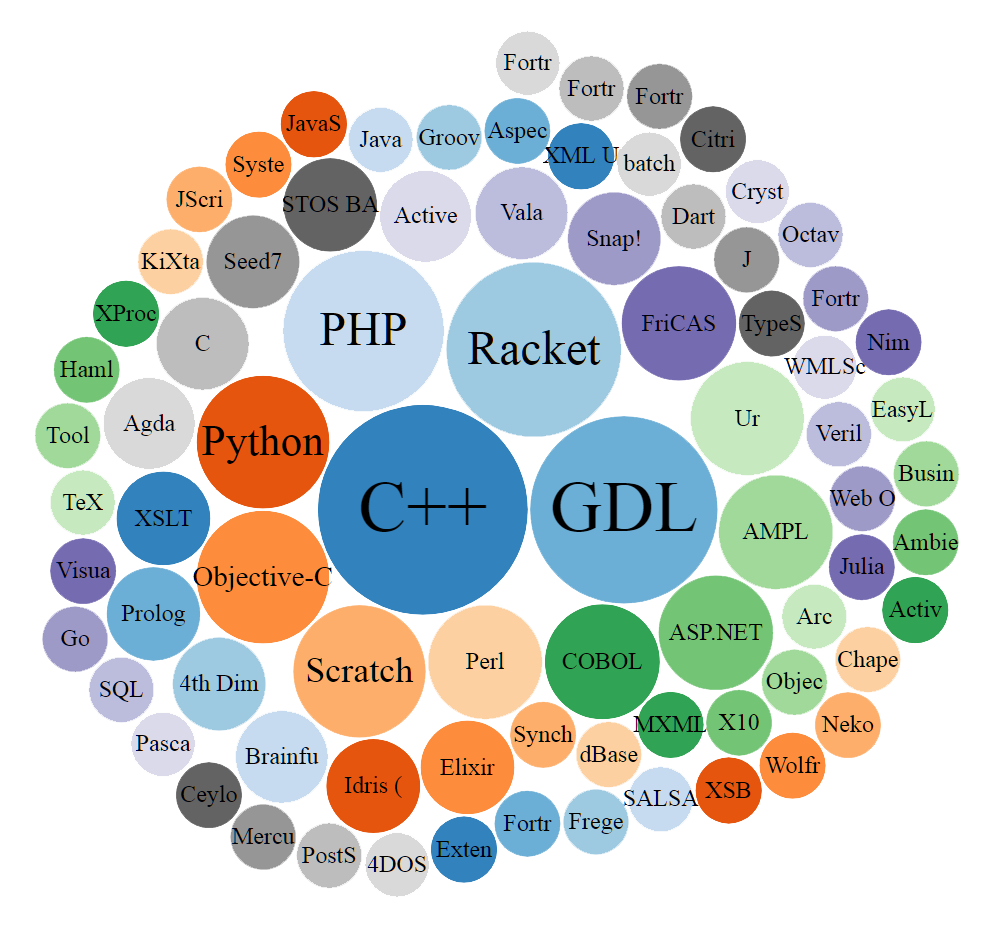
\includegraphics[width=0.8\linewidth]{./chapter/programming_language/File_extensions_quantity_of_source_code_2017.png}
	\label{fig:source_format_2017}
    \caption[Пузырьковая диаграмма по числу форматов файлов исходного кода для разных языков программирования на 2017 год]{Пузырьковая диаграмма по числу форматов файлов исходного кода для разных языков программирования на 2017 год. Размер пузырька соответствует числу форматов для одного языка. Ссылка на SPARQL-запрос: \href{https://w.wiki/uGQ}{https://w.wiki/uGQ}}
\end{figure}
К 2020 году (рис.~\ref{fig:source_format_2020}) \href{https://en.wikipedia.org/wiki/C++}{C++} и \href{https://en.wikipedia.org/wiki/Geometric_Description_Language}{Geometric Description Language (GDL)} остались на лидирующем месте (10 и 8 форматов-расширений). За три года подтянулись и вошли в первую восьмёрку также такие языки, как \href{https://ru.wikipedia.org/wiki/Racket_(язык_программирования)}{Racket}, \href{https://en.wikipedia.org/wiki/Raku_(programming_language)}{Raku} (9 форматов), \href{https://en.wikipedia.org/wiki/Rexx}{REXX} и \href{https://en.wikipedia.org/wiki/Scratch_(programming_language)}{Scratch} (по 6 форматов), \href{https://ru.wikipedia.org/wiki/Java}{Java} и \href{https://en.wikipedia.org/wiki/Wolfram_Language}{Wolfram Language} (по 5 форматов).
\begin{figure}
\centering
	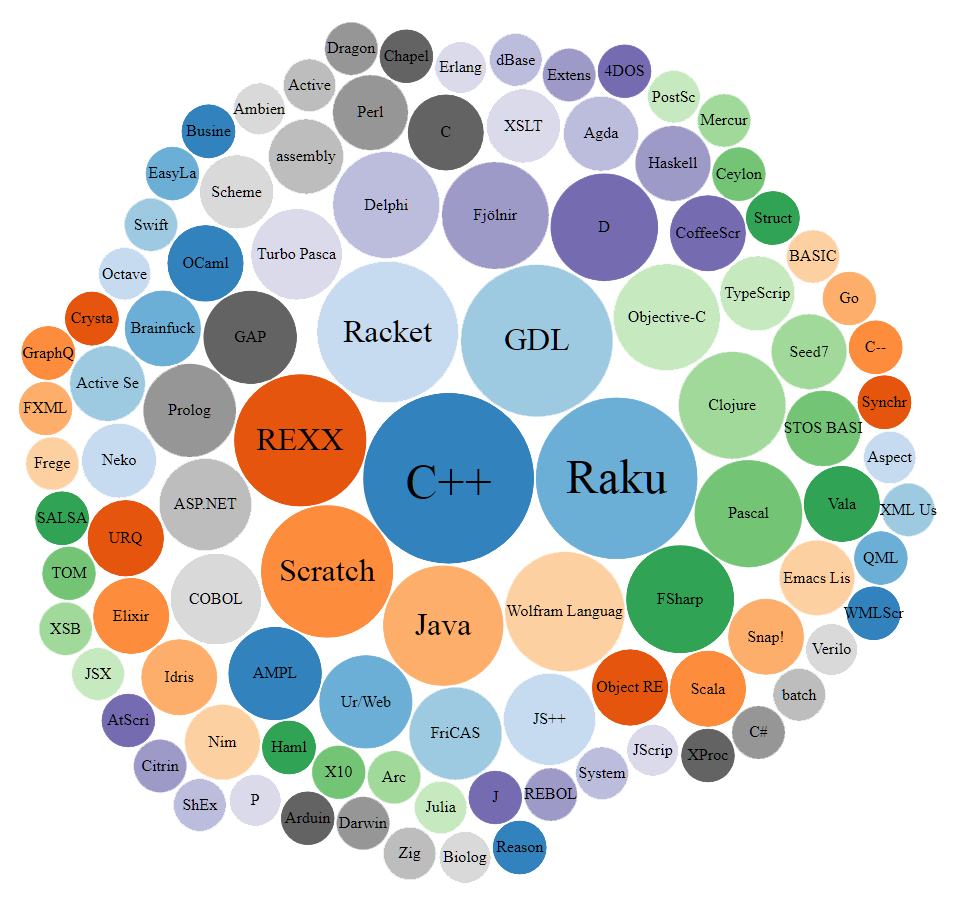
\includegraphics[width=0.8\linewidth]{./chapter/programming_language/File_extensions_quantity_of_source_code_2020.png}
	\label{fig:source_format_2020}
	\caption{Пузырьковая диаграмма по числу форматов файлов исходного кода для 108 языков программирования на 2020 год. Размер пузырька соответствует числу форматов для одного языка. Ссылка на SPARQL-запрос: \href{https://w.wiki/uGQ}{https://w.wiki/uGQ}}
\end{figure}

\footnotetext{Рисунки~\ref{fig:source_format_2017} и ~\ref{fig:source_format_2020} построены при при помощи запроса~\ref{lst:source_formats}.}
Из этого можно сделать вывод, что развитие языков программирования продолжается непрерывно, постоянно возникают новые форматы файлов исходного кода, но лидеры по числу расширений файлов с трудом могут уступать лидирующие позиции. Это может быть связано с тем, что раз возникнув, языку уже трудно избавиться от расширения, ввиду потери совместимости с более ранними версиями языка. Таким образом наличие множества расширений, скорее, указывает на отсутствие единого стандарта и строгих правил на первых порах.

%%
% Страны, в которых живут люди и располагаются организации, связанные с созданием языков программирования
%%
\section{Страны, в которых располагаются организации и проживают люди, связанные с разработкой языков программирования}

Отобразим на карте мира те страны, в которых живут люди и располагаются организации, связанные с созданием языков программирования. Заметим, что разработчиком языка (свойство: \href{https://www.wikidata.org/wiki/Property:P178}{developer (P178)}, см.~листинг~\ref{lst:countries_map}) может выступать как организация, так и отдельный человек (далее по тексту под "разработчиком" понимается одно из двух этих понятий). Для определения месторасположения (свойство: \href{https://www.wikidata.org/wiki/Property:P625}{coordinate location (P625)}) организации будем использовать координаты её штаб-квартиры (свойство: \href{https://www.wikidata.org/wiki/Property:P159}{headquarters location (P159)}), для человека~--- координаты места его рождения (свойство: \href{https://www.wikidata.org/wiki/Property:P19}{place of birth (P19)}).

\footnotetext{Результатом запроса~\ref{lst:countries_map} является карта, где красными точками указаны места проживания людей или штабы фирм, причастных к разработке языков программирования. На рисунке рис.~\ref{fig:countries_2017} изображен результат запроса на 2017 год, а на рис.~\ref{fig:countries_2020} показаны аналогичные данные на 2020 год.}
\index{График!Map!Карта с указанием места жительства или работы разработчиков языков программирования}
\begin{lstlisting}[
	language=SPARQL,
	label=lst:countries_map,
	caption={\href{https://w.wiki/v3b}{Карта с указанием места жительства или работы разработчиков языков программирования}\protect\footnotemark},
	texcl
]
#defaultView:Map
SELECT ?lang_label ?developerLabel ?locationLabel ?coord
WHERE
{
   ?lang wdt:P31 wd:Q9143. # instances of programming language
   ?lang wdt:P178 ?developer. # developer
   { ?developer wdt:P159 ?location. } UNION # headquarters location
   { ?developer wdt:P19 ?location. } # place of birth
   ?location wdt:P625 ?coord. # coordinate location
   SERVICE wikibase:label { bd:serviceParam wikibase:language "ru" } 	
}
\end{lstlisting}

\begin{figure}[h]
\centering
	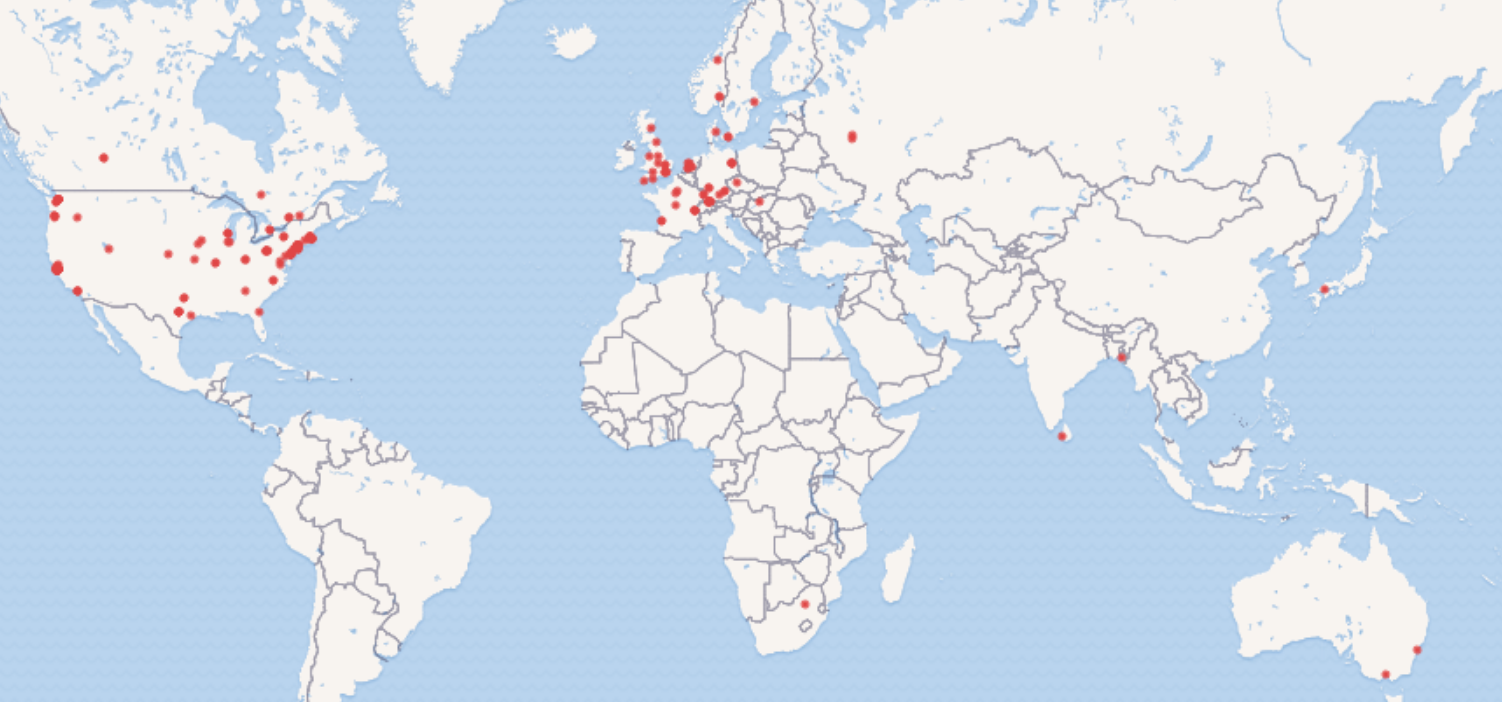
\includegraphics[width=1\textwidth]{./chapter/programming_language/Map_showing_contries_2017.png}
	\caption{Страны, в которых живут люди или расположены организации, связанные с созданием языков программирования, 2017 год. Ссылка на SPARQL-запрос: \href{https://w.wiki/v3b}{https://w.wiki/v3b}}
	\label{fig:countries_2017}
\end{figure}
\begin{figure}
\centering
	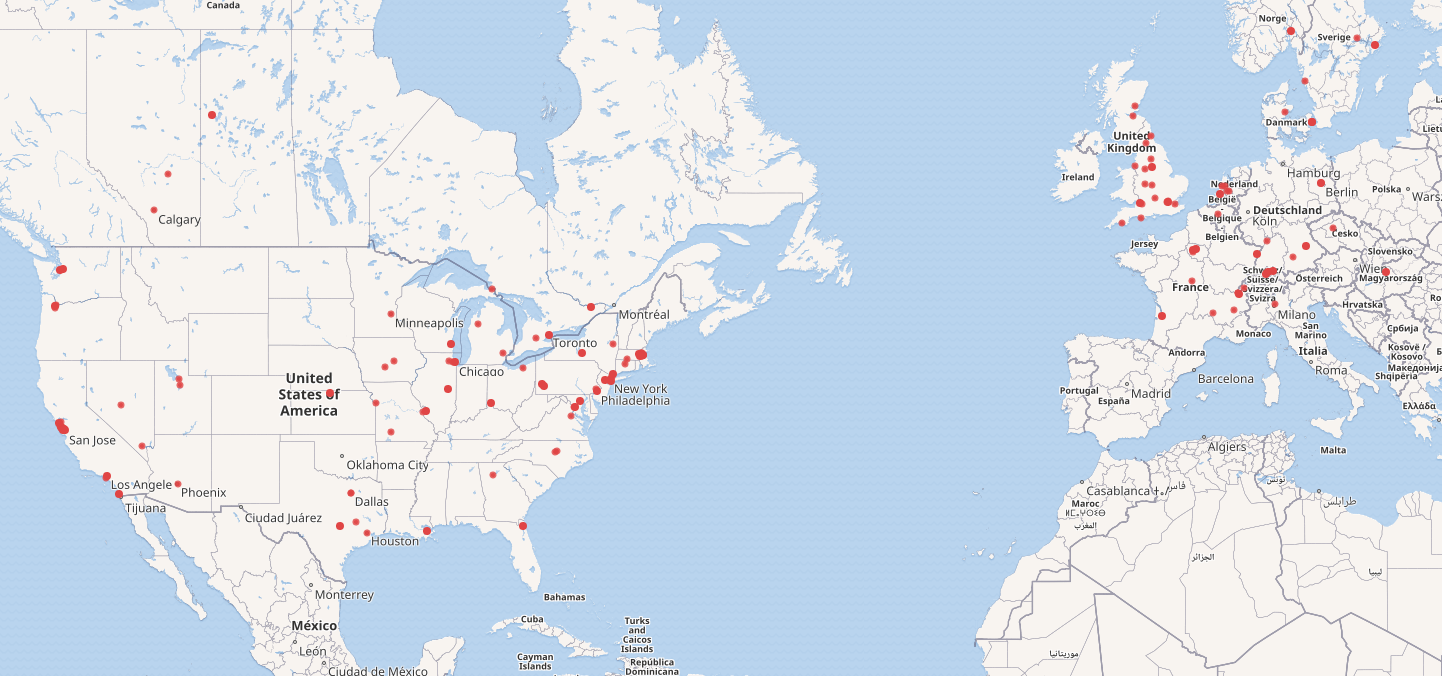
\includegraphics[width=1\textwidth]{./chapter/programming_language/Map_showing_contries_2020.png}
	\caption{Страны, в которых живут люди или расположены организации, связанные с созданием языков программирования, 2020 год. Ссылка на SPARQL-запрос: \href{https://w.wiki/v3b}{https://w.wiki/v3b}}
	\label{fig:countries_2020}
\end{figure}

\begin{marginfigure}
{
\setlength{\fboxsep}{0pt}%
\setlength{\fboxrule}{1pt}%
\fcolorbox{white}{white}{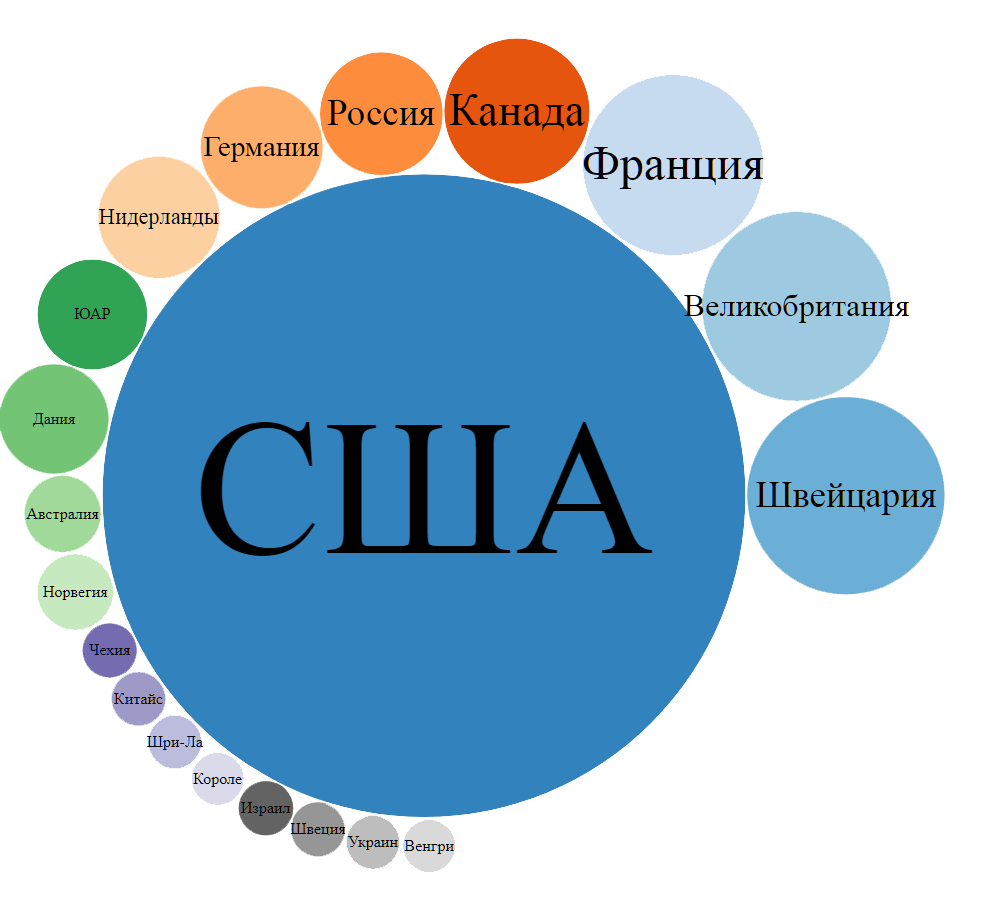
\includegraphics[width=\linewidth]{./chapter/programming_language/The_most_favorable_countries_for_the_emergence_of_people_capable_of_developing_programming_languages_2020_RU.png}}
}
  \caption{Наиболее благоприятные страны для появления людей, способных к разработке языков программирования на 2020 год. Размер пузырька соответствует числу людей, причастных к разработке языков программирования, из соответствующей страны. Ссылка на SPARQL-запрос: \href{https://w.wiki/v3s}{https://w.wiki/v3s}}%
  \label{fig:countries_2_2020}%
\end{marginfigure}
По  рис.~\ref{fig:countries_2017} и рис.~\ref{fig:countries_2020} можно сделать вывод, что наиболее благоприятными местами жительства для людей, разрабатывающих языки программирования, являются восточное побережье \href{https://en.wikipedia.org/wiki/USA}{США}, \href{https://ru.wikipedia.org/wiki/Центральная_Европа}{Центральная Европа} и \href{https://ru.wikipedia.org/wiki/Великобритания}{Великобритания}.

Построим (листинг~\ref{lst:countries_bubble}) также пузырьковую диаграмму, чтобы выявить наиболее благоприятные страны для появления людей, способных к разработке языков программирования и размещению в этих странах штаб-квартир. 
\index{График!BubbleChart!Пузырьковая диаграмма благоприятных стран для появления разработчиков языков программирования}
\begin{lstlisting}[
	language=SPARQL,
	label=lst:countries_bubble,
	caption={\href{https://w.wiki/v3s}{Пузырьковая диаграмма благоприятных стран для появления разработчиков языков программирования}\protect\footnotemark},
	texcl
]
#defaultView:BubbleChart
SELECT ?stateLabel (count(*) as ?count)
WHERE {
  ?lang wdt:P31 wd:Q9143. # instances of programming language
  ?lang wdt:P178 ?developer. # developer
  ?developer rdfs:label ?developerLabel. 
  { ?developer wdt:P159 ?location. } UNION # headquarters location
  { ?developer wdt:P19 ?location. } # place of birth
  ?location wdt:P17 ?state.
  SERVICE wikibase:label { bd:serviceParam wikibase:language "ru" } 	
}
GROUP BY ?stateLabel
ORDER BY DESC(?count)
\end{lstlisting}

Видим на рис.~\ref{fig:countries_2_2020}, что наиболее благоприятными странами оказались \href{https://en.wikipedia.org/wiki/USA}{США} (241 человек и штаб-квартир), \href{https://ru.wikipedia.org/wiki/Великобритания}{Великобритания} (24), \href{https://ru.wikipedia.org/wiki/Франция}{Франция}, тогда как в России подобных штаб-квартир~--- 5. Также в \href{https://en.wikipedia.org/wiki/Russia}{России} было разработано только два языка программирования: \href{https://www.wikidata.org/wiki/Q2626418}{РЕФАЛ} (1966 год) и \href{https://www.wikidata.org/wiki/Q65065977}{встроенный язык программирования 1С:Предприятие} (1996 год).

На 2020 год (рис.~\ref{fig:countries_2_2020}) число штаб-квартир в США равно 241, в Великобритании — 24, во Франции — 18 и в России — 5.

%%
% Университеты, в которых учились люди, разрабатывавшие языки программирования
%%
\section{Университеты, в которых учились разработчики языков программирования}
Отобразим (листинг~\ref{lst:developer_university}) на карте учебные заведения, в которых учились студенты, впоследствии разработавшие языки программирования.

\footnotetext{Результатом запроса~\ref{lst:developer_university} будет карта, на которой красными точками отмечены места расположения университетов, в которых учились люди, создавшие языки программирования. На 2017 год получено 142 университета, к 2020 число записей увеличилось до 282.}
\index{График!Map!Карта с указанием университетов, в которых учились разработчики языков программирования}
\begin{lstlisting}[
	language=SPARQL,
	label=lst:developer_university,
	caption={\href{https://w.wiki/v3v}{Карта с указанием университетов, в которых учились разработчики языков программирования}\protect\footnotemark},
	texcl
]
#defaultView:Map
SELECT ?langLabel ?developerLabel ?educational_institutionLabel ?coord
WHERE {
  ?lang wdt:P31 wd:Q9143. # instances of programming language
  ?lang wdt:P178 ?developer. # developer
  ?developer wdt:P69 ?educational_institution. # educated at
  ?educational_institution wdt:P625 ?coord. # coordinate location
  SERVICE wikibase:label { bd:serviceParam wikibase:language "ru" } 	
}
\end{lstlisting}

\begin{figure}[h]
\centering
	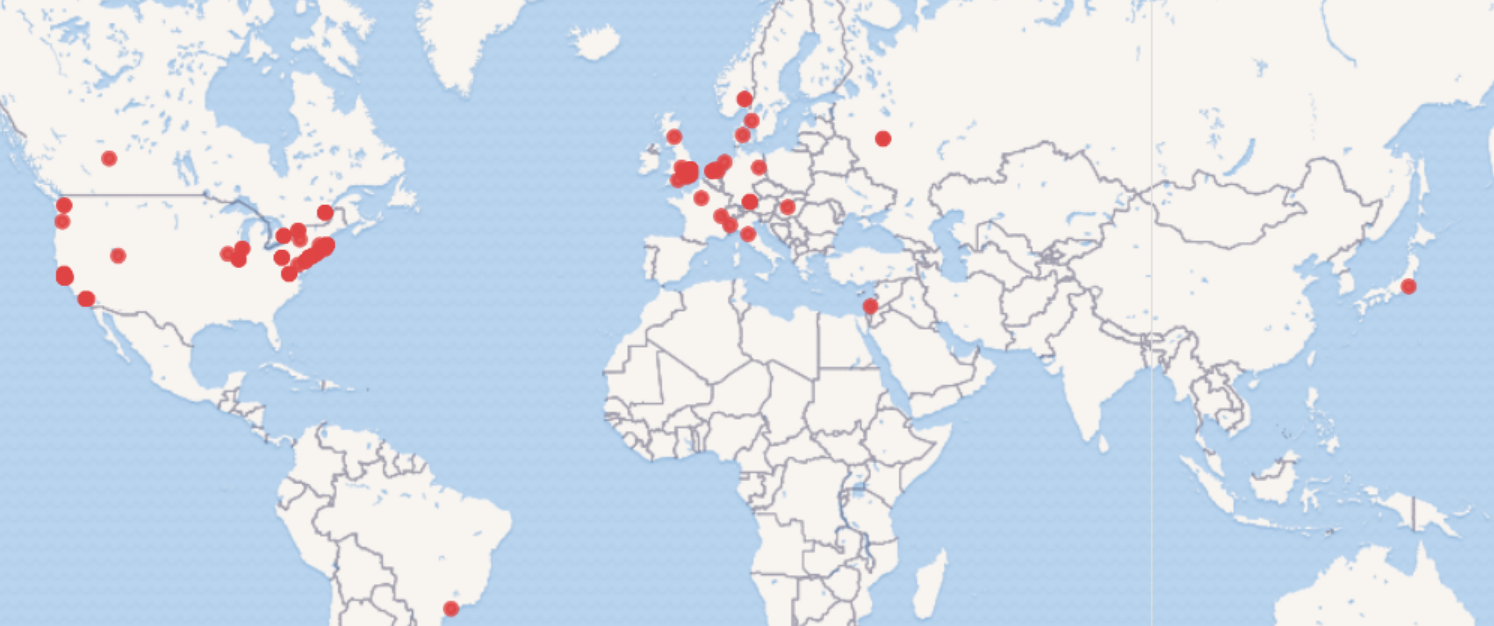
\includegraphics[width=1\textwidth]{./chapter/programming_language/Map_showing_educational_institutes_2017.png}
	\caption{Учебные заведения, в которых учились разработчики языков программирования, 2017 год. Ссылка на SPARQL-запрос: \href{https://w.wiki/uGb}{https://w.wiki/uGb}}
	\label{fig:universities_2017}
\end{figure}
\begin{figure}[h]
\centering
	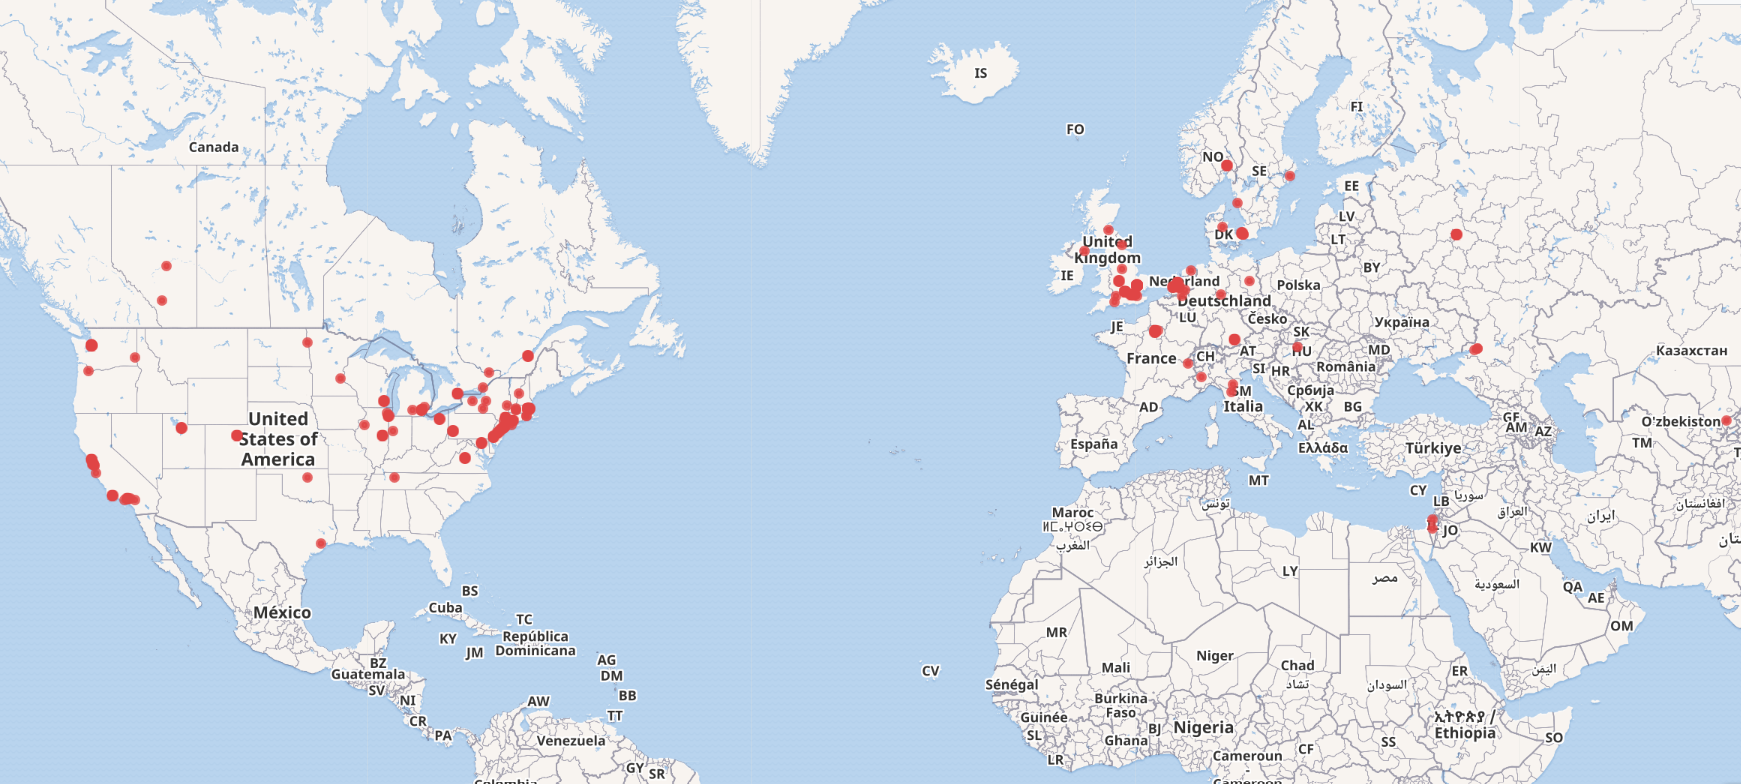
\includegraphics[width=1\textwidth]{./chapter/programming_language/Map_showing_educational_institutes_2020.png}
	\caption{Учебные заведения, в которых учились разработчики языков программирования, 2020 год. Ссылка на SPARQL-запрос: \href{https://w.wiki/uGb}{https://w.wiki/uGb}}
	\label{fig:universities_2020}
\end{figure}
\marginnote{Сколько языков программирования появилось за последние три года? В каком году было изобретено максимальное число языков?}

По картам~\ref{fig:universities_2017} и~\ref{fig:universities_2020} видно, что большая часть людей, причастных к созданию языков программирования, учились в Европе или в США и динамика не сильно изменилась за 3 года.

Построим также пузырьковую диаграмму (листинг~\ref{lst:developer_universities_bubble}) по самым популярным учебным заведениям для обучения, среди будущих создателей языков программирования. На первых местах по числу обучающихся разработчиков оказались: \href{https://www.wikidata.org/wiki/Q21578}{Принстонский университет} (8 студентов) и \href{https://www.wikidata.org/wiki/Q41506}{Стэнфордский университет} (8). \href{https://ru.wikipedia.org/wiki/Московский_государственный_университет}{Московский государственный университет} оказался в конце списка, в нём учился \href{https://www.wikidata.org/wiki/Q92602}{Энтони Ричард Хоар}, разработавший \href{https://www.wikidata.org/wiki/Q188436}{ALGOL60} (1958 год), и \href{https://www.wikidata.org/wiki/Q4466506}{Валентин Фёдорович Турчин}, разработавший \href{https://www.wikidata.org/wiki/Q2626418}{РЕФАЛ}. Список, в который попал МГУ, содержит 142 вуза мира.

\index{График!BubbleChart!Университеты, в которых учились разработчики языков программирования}
\begin{lstlisting}[
	language=SPARQL,
	label=lst:developer_universities_bubble,
	caption={\href{https://w.wiki/uGc}{Университеты, в которых учились разработчики языков программирования}\protect\footnotemark},
	texcl
]
#defaultView:BubbleChart
SELECT ?educationalInstitutionLabel (count(*) as ?count)
WHERE {
 ?lang wdt:P31 wd:Q9143. # instances of programming language
 ?lang wdt:P178 ?developer. # developer
 ?developer wdt:P69 ?educationalInstitution. # educated at
 ?educationalInstitution wdt:P625 ?coord. # coordinate location
 SERVICE wikibase:label { bd:serviceParam wikibase:language "ru" } 	
}
GROUP BY ?educationalInstitutionLabel
ORDER BY DESC(?count)
\end{lstlisting}

%%
% Профессии создателей языков программирования
%%
\section{Профессии создателей языков программирования}

\begin{marginfigure}[-102pt]
{
\setlength{\fboxsep}{0pt}
\setlength{\fboxrule}{1pt}
\fcolorbox{white}{white}{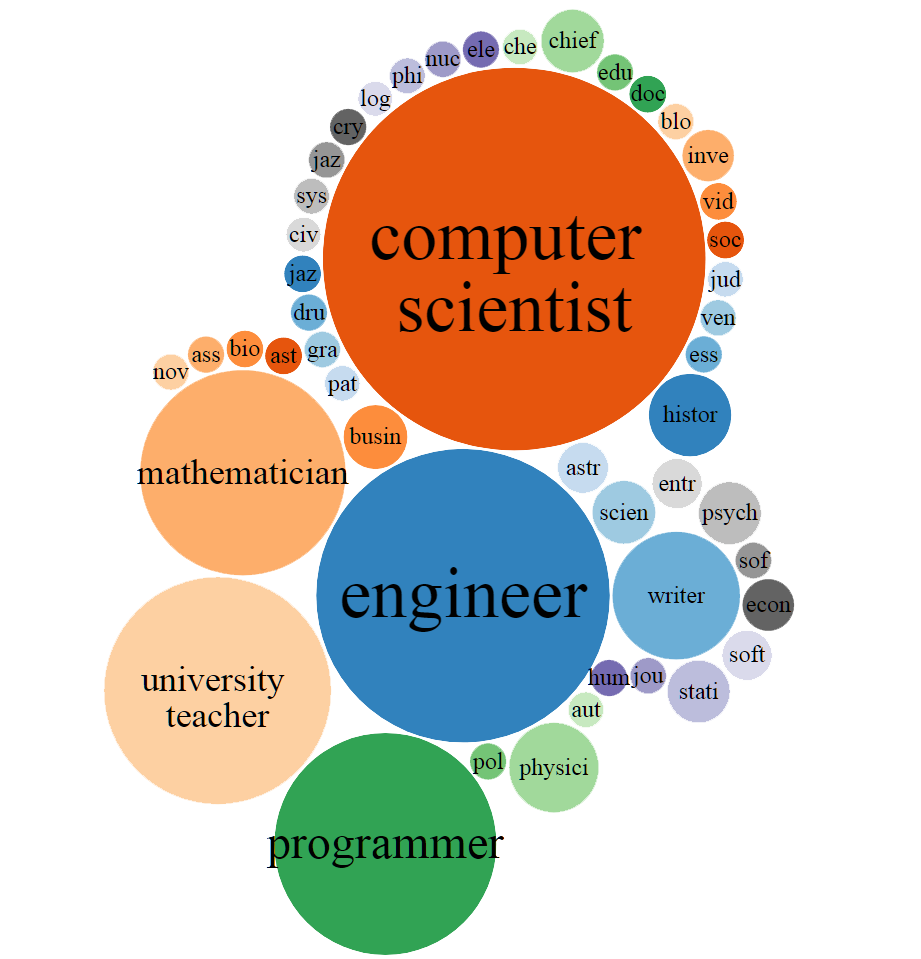
\includegraphics[width=\linewidth]{./chapter/programming_language/Bubble_chart_showing_the_quantity_of_professions_people_,creating_programming_languages,_have_2017.png}}
}
  \caption{Профессии разработчиков языков программирования, 2017 год. Размер пузырька показывает число разработчиков с соответствуюшей профессией.}
  \label{fig:2017_profession}
\end{marginfigure}
\begin{marginfigure}[-2pt]
{
\setlength{\fboxsep}{0pt}
\setlength{\fboxrule}{1pt}
\fcolorbox{white}{white}{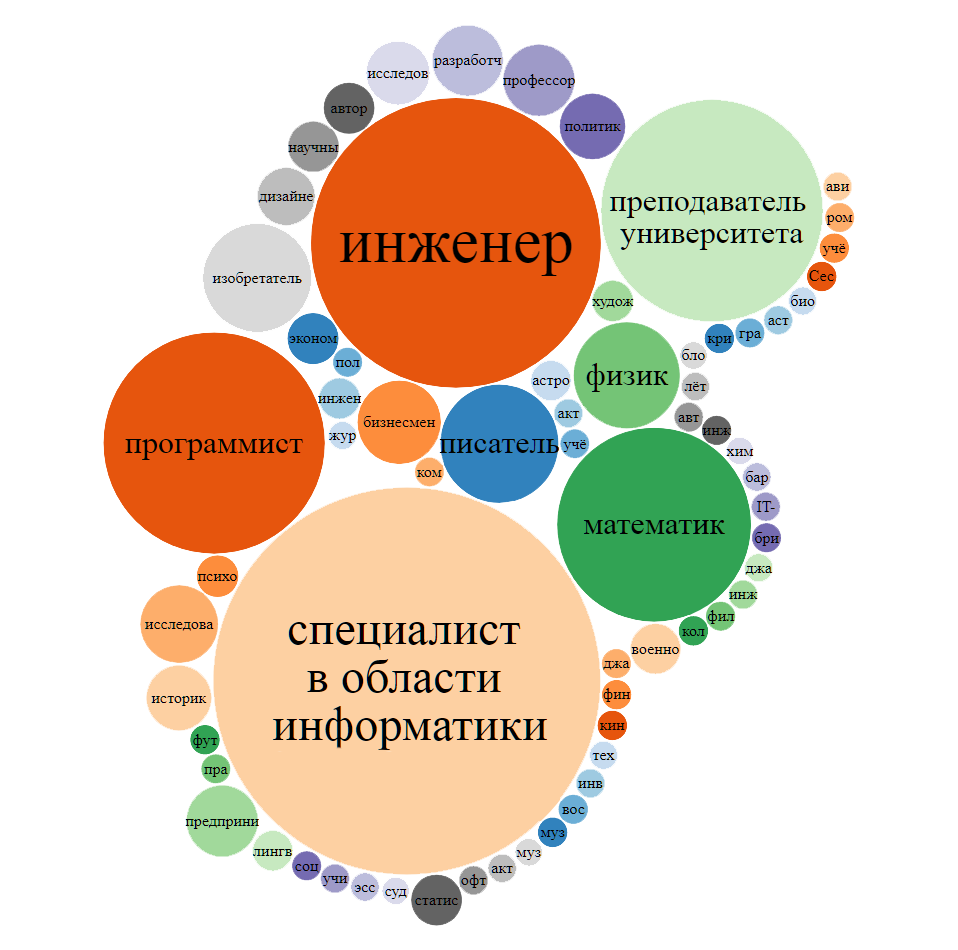
\includegraphics[width=\linewidth]{./chapter/programming_language/Bubble_chart_showing_the_quantity_of_professions_people,_creating_programming_languages_RU_2020.png}}
}
  \caption{Профессии разработчиков языков программирования программирования, 2020 год. Размер пузырька показывает число разработчиков с соответствуюшей профессией.}
  \label{fig:2020_profession}
\end{marginfigure}
Построим пузырьковую диаграмму (листинг~\ref{lst:developer_profession}), отображающую информацию о том, какие профессии преобладают среди людей, разрабатывающих языки программирования.
\index{График!BubbleChart!Профессии создателей языков программирования}
\begin{lstlisting}[
	language=SPARQL,
	label=lst:developer_profession,
	caption={\href{https://w.wiki/v42}{Профессии создателей языков программирования}\protect\footnotemark},
	texcl
]
#defaultView:BubbleChart
SELECT ?occupationLabel (count(*) as ?occupation)
WHERE {
  ?lang wdt:P31 wd:Q9143. # instances of programming language 
  ?lang wdt:P178 ?developer. # developer
  ?developer wdt:P106 ?occupation. # occupation
  SERVICE wikibase:label { bd:serviceParam wikibase:language "ru" }
}
GROUP BY ?occupationLabel 
ORDER BY DESC(?count)
\end{lstlisting}
\footnotetext{Получено 48 профессий в 2017 году и 74 профессии в 2020 году. Ссылка на SPARQL-запрос: \href{https://w.wiki/v42}{https://w.wiki/v42}}

Результаты запроса~\ref{lst:developer_profession} в 2017 и 2020 годах можно видеть на рисунках~\ref{fig:2017_profession} и~\ref{fig:2020_profession} соответственно.
\marginnote{Герберт Александер Саймон (1916--2001 годы), разработчик \href{https://en.wikipedia.org/wiki/Information_Processing_Language}{Языка обработки информации (IPL)}}
Наиболее распространенными профессиями оказались: \href{https://www.wikidata.org/wiki/Q21198}{специалист в области компьютерных наук}, \href{https://www.wikidata.org/wiki/Q81096}{инженер} и \href{https://www.wikidata.org/wiki/Q37226}{учитель}. Интересно заметить, что встречаются такие профессии как джазовый музыкант и политик. Например, обеими этими профессиями владел \href{https://www.wikidata.org/wiki/Q181529}{Герберт Александер Саймон}. На 2020 год среди разработчиков языков программирования оказалось больше всего специалистов в области компьютерных наук (172 человека), а также 96 инженеров, 57 учителей, 56 программистов и 43 математика.

%%
% Объектно-ориентированные языки программирования
%%
\section{Объектно-ориентированные языки программирования}
Получим список всех объектно-ориентированных языков программирования (листинг~\ref{lst:oopl}).

\begin{lstlisting}[
	language=SPARQL,
	label=lst:oopl,
	caption={\href{https://w.wiki/v47}{Список объектно-ориентированных языков программирования}\protect\footnotemark},
	texcl
]
SELECT DISTINCT ?lang ?langLabel
WHERE {
 ?lang wdt:P31 wd:Q899523 # instances of object-oriented programming language
 SERVICE wikibase:label { bd:serviceParam wikibase:language "ru" }
}
\end{lstlisting}
\footnotetext{Результатом SPARQL-запроса~\ref{lst:oopl} является список объектно-ориентированных языков программирования. На 2017 год список содержал 116 записей, к 2020 году число записей увеличилось на 2 и составляет 118 языков программирования. Ссылка на SPARQL-запрос: \href{https://w.wiki/v47}{https://w.wiki/v47}}

Таким образом 8\% языков программирования на 2020 год являются объектно-ориентированными (отношение числа объектно-ориентированных языков программирования(листинг~\ref{lst:oopl}, 118 языков) ко всем языкам программирования (листинг~\ref{lst:prog_langs}, 1422 языка)).

%%
% Полнота викиданных
%%
\section{Полнота языков программирования в Викиданных}
По данным Боровского исследовательского университета\cite{oo_langs_bourabai} существует, как минимум, 26 языков программирования, которые поддерживают объектно-ориентированную парадигму. В статьях посвящённых объектно-ориентированному программированию к этому списку добавляются ещё 4\cite{oo_langs_science_wikia} и 3\cite{oo_langs_garshin} языка программирования. При этом SPARQL-запрос~\ref{lst:oopl} вернул 118 результатов.

Судить о полноте данных по трём приведённым выше источникам достаточно сложно, так как в них обсуждается большое количество малоизвестных, устаревших и узконаправленных языков, которые не освещаются в авторитетных источниках, и при этом не рассматириваются недавно возникшие языки программирования. Таким образом можно предположить, что Викиданные предоставляют достаточно полный список объектно-ориентированных языков программирования.

%%
% Степень заполненности объектов
%%
\section{Степень заполненности объектов разработчиков языков программирования}
Выведем список разработчиков, у объектов которых заполнено поле label (листинг~\ref{lst:filling}).

\begin{lstlisting}[
	language=SPARQL,
	label=lst:filling,
	caption={\href{https://w.wiki/v4L}{Список разработчиков языков программирования с заполненным полем label}\protect\footnotemark},
	texcl
]
SELECT ?itemLabel ?item ?developerLabel ?developer
WHERE {
  ?item wdt:P31 wd:Q9143 # instances of programming language
  ?item wdt:P178 ?developer. # developer 
  ?developer wdt:P31 wd:Q5. # instances of human
  SERVICE wikibase:label { bd:serviceParam wikibase:language "ru" }
}
\end{lstlisting}
\footnotetext{Результатом запроса в 2017 году было 133 разработчика, в 2020 году получено 237 разработчика. Ссылка на SPARQL-запрос: \href{https://w.wiki/v4L}{https://w.wiki/v4L}}
Сравнив результаты рапросов, можно заметить, что число объектов в Викиданных растёт и степень их заполненности также увеличивается.

%%
% Упражнения
%%
\section{Упражнения}
\label{prog_lang_test}
\marginnote{\index{Языки программирования!Определения!Хештег}Хештег (\#)~--- ключевое слово или несколько слов сообщения, тег (пометка), используемый в микроблогах и социальных сетях, облегчающий поиск сообщений по теме или содержанию и начинающийся со знака решётки.}
\begin{enumerate}
	\itemВывести все языки программирования со свойством <<\href{https://www.wikidata.org/wiki/Property:P822}{персонаж-талисман (P822)}>> (узнаваемый персонаж, олицетворяющий собой некий коллектив: школу, спортивную команду, сообщество, воинское подразделение, мероприятие или бренд).
Ответ можно найти на странице~\pageref{answer:prog_langs_4}.
	\itemПодчитать количество языков программирования, созданных ранее 1992 года (используйте свойство: <<\href{https://www.wikidata.org/wiki/Property:P571}{дата-основания/создания (P571)}>>).
Ответ можно найти на странице~\pageref{answer:prog_langs_4}.
	\itemПостроить столбчатую диаграмму, отражающую количество известных хештегов в Твиттере для каждого языка программирования (свойство: <<\href{https://www.wikidata.org/wiki/Property:P2572}{хештег Твиттера (P2572)}>>).
Ответ можно найти на странице~\pageref{answer:prog_langs_4}.
\end{enumerate}
